\documentclass[tikz]{standalone}
\usepackage{tikz}
\usepackage{amsmath}
\usepackage{amsfonts}
\usetikzlibrary{arrows.meta, calc}

% The columns of A, and the basis they replace.
\colorlet{colcolor}{red!60!orange}
\colorlet{basiscolor}{blue!50!cyan}

\begin{document}
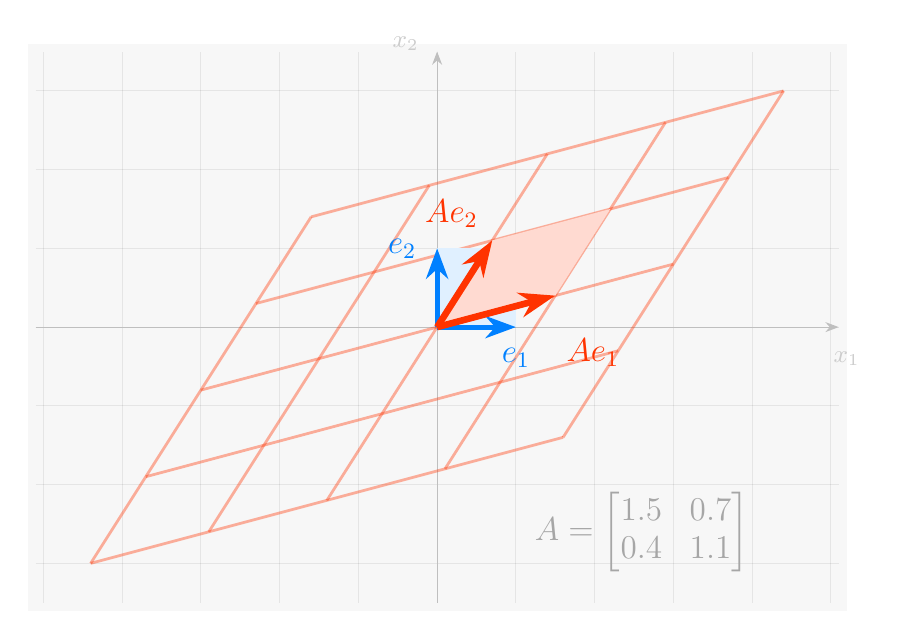
\begin{tikzpicture}[>=Stealth]

  % Frame 10.4 wide by 7.2 tall, matching the 1.45 proportion of the other covers.
  \fill[gray!6] (-5.2,-3.6) rectangle (5.2,3.6);

  % The space before the matrix acts: faint unit grid.
  \begin{scope}[opacity=0.07]
    \foreach \x in {-5,...,5} { \draw[black, thin] (\x,-3.5) -- (\x,3.5); }
    \foreach \y in {-3,...,3} { \draw[black, thin] (-5.1,\y) -- (5.1,\y); }
  \end{scope}

  \draw[->, black!25, thin] (-5.1,0) -- (5.1,0);
  \draw[->, black!25, thin] (0,-3.5) -- (0,3.5);
  \node[black!20, font=\small] at (5.2,-0.4) {$x_1$};
  \node[black!20, font=\small] at (-0.4,3.6) {$x_2$};

  % A = [[1.5, 0.7], [0.4, 1.1]]. TikZ's cm={a,b,c,d} maps
  % (x,y) -> (ax+cy, bx+dy), so a=A11 b=A21 c=A12 d=A22.
  % The grid runs to +-2, which A sends to +-4.4 by +-3.0: inside the frame.
  \begin{scope}[cm={1.5, 0.4, 0.7, 1.1, (0,0)}, opacity=0.38]
    \foreach \x in {-2,...,2} { \draw[colcolor, line width=1.0pt] (\x,-2) -- (\x,2); }
    \foreach \y in {-2,...,2} { \draw[colcolor, line width=1.0pt] (-2,\y) -- (2,\y); }
  \end{scope}

  % The unit square, and where the matrix sends it.
  \fill[basiscolor!12] (0,0) -- (1,0) -- (1,1) -- (0,1) -- cycle;
  \fill[colcolor!18] (0,0) -- (1.5,0.4) -- (2.2,1.5) -- (0.7,1.1) -- cycle;

  \draw[basiscolor, line width=1.8pt, -{Stealth[length=11pt, width=8pt]}] (0,0) -- (1,0);
  \draw[basiscolor, line width=1.8pt, -{Stealth[length=11pt, width=8pt]}] (0,0) -- (0,1);
  \node[basiscolor, font=\large\bfseries\sffamily, anchor=north] at (1.0,-0.14) {$e_1$};
  \node[basiscolor, font=\large\bfseries\sffamily, anchor=east] at (-0.14,1.0) {$e_2$};

  \draw[colcolor, line width=2.4pt, -{Stealth[length=13pt, width=9pt]}] (0,0) -- (1.5,0.4);
  \draw[colcolor, line width=2.4pt, -{Stealth[length=13pt, width=9pt]}] (0,0) -- (0.7,1.1);
  \node[colcolor, font=\large\bfseries\sffamily, anchor=north west] at (1.52,-0.03) {$Ae_1$};
  \node[colcolor, font=\large\bfseries\sffamily, anchor=south east] at (0.64,1.14) {$Ae_2$};

  \node[black!35, font=\large\sffamily] at (2.6,-2.6)
    {$A = \begin{bmatrix} 1.5 & 0.7 \\ 0.4 & 1.1 \end{bmatrix}$};

\end{tikzpicture}
\end{document}
